\section{motor\_\-pwm.h File Reference}
\label{motor__pwm_8h}\index{motor_pwm.h@{motor\_\-pwm.h}}


This graph shows which files directly or indirectly include this file:\begin{figure}[H]
\begin{center}
\leavevmode
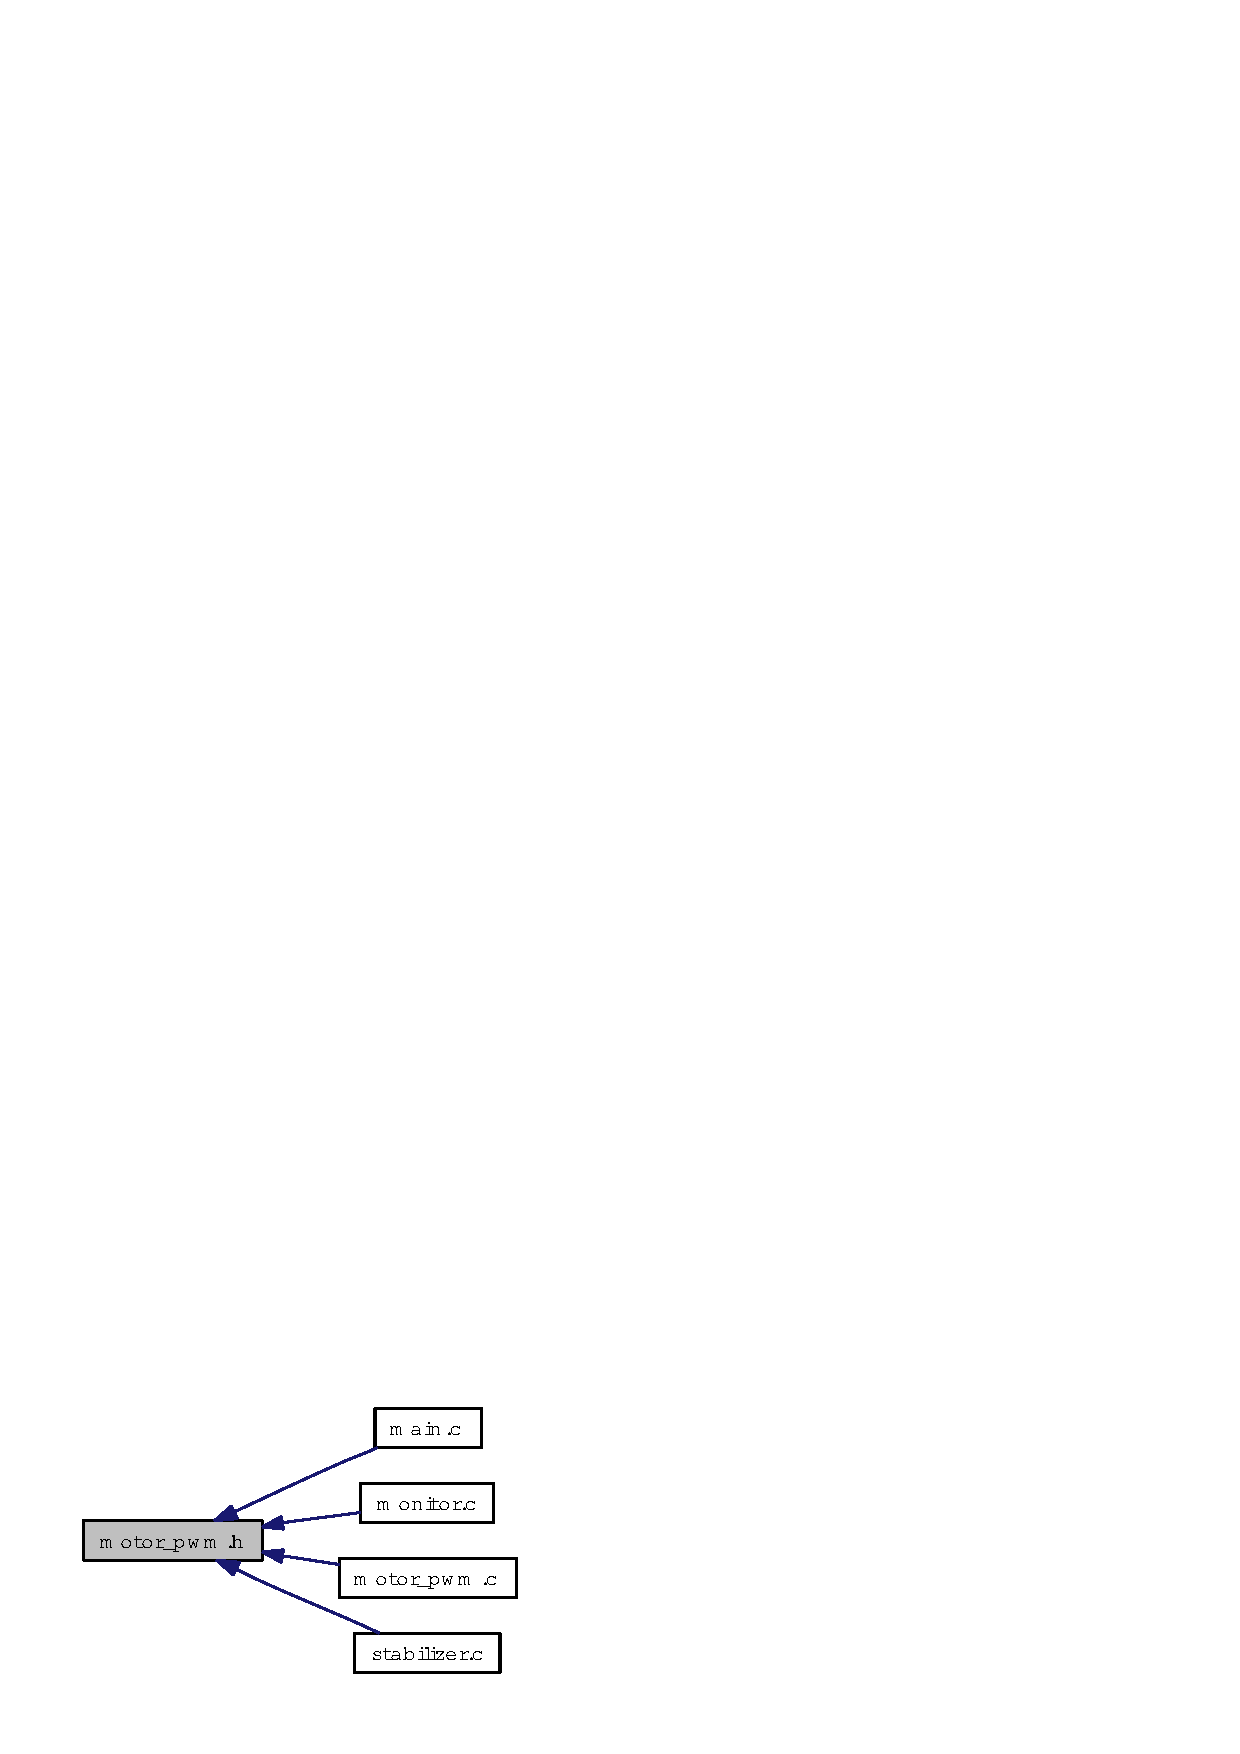
\includegraphics[width=126pt]{motor__pwm_8h__dep__incl}
\end{center}
\end{figure}
\subsection*{Defines}
\begin{CompactItemize}
\item 
\#define {\bf PWM\_\-RESOLUTION}~255
\item 
\#define {\bf PWM\_\-SECURITY\_\-MAX\_\-FREQ}~10000
\item 
\#define {\bf PWM\_\-SECURITY\_\-MIN\_\-DUTY}~(PWM\_\-RESOLUTION / 200)
\end{CompactItemize}
\subsection*{Functions}
\begin{CompactItemize}
\item 
void {\bf init\_\-motor\_\-pwm} (void)
\item 
void {\bf set\_\-motor\_\-pwm\_\-freq} (uint16\_\-t hz)
\item 
void {\bf enable\_\-motor1} (void)
\item 
void {\bf enable\_\-motor2} (void)
\item 
void {\bf disable\_\-motor1} (void)
\item 
void {\bf disable\_\-motor2} (void)
\item 
void {\bf set\_\-motor1} (uint8\_\-t speed, uint8\_\-t dir)
\item 
void {\bf set\_\-motor2} (uint8\_\-t speed, uint8\_\-t dir)
\end{CompactItemize}
\subsection*{Variables}
\begin{CompactItemize}
\item 
uint8\_\-t {\bf \_\-\_\-motor1\_\-duty}
\item 
uint8\_\-t {\bf \_\-\_\-motor2\_\-duty}
\end{CompactItemize}
